\subsection{Session 3, Exercise 3}

\lineparagraph{Exercise}

Is the language regular, that consists of sequences of $0$'s of a length that is...
\begin{enumerate}[a.)]
\item an even number?
\item an odd number?
\item a perfect square?
\item a power of $2$?
\end{enumerate}

\lineparagraph{Solution}

\subsubsection{Even number of 0's}

Regular.

\textbf{Proof 1}: The regular expression $(00)^*$ matches them.

Proof that this regular expression matches the language:

\begin{itemize}
    \item The $^*$ operator allows any number of repeats, even 0.
    \item Inside the $^*$ operator we have two $0$'s, which can be repeated any number of times to match any even number of $0$'s.
    \item The empty string, also known as zero number of $0$'s contains an even number of $0$'s, so it is part of the language. $(00)^*$ matches the empty string, which is correct.
\end{itemize}

\textbf{Proof 2}: The following DFA accepts the language:

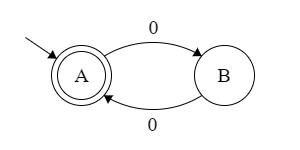
\includegraphics[width=150px]{03/even_zeroes.png}

Proof that this automaton accepts the language:

\begin{itemize}
    \item Words that end up in state $A$ are the words that contain an even number of $0$'s, while words that end up in state $B$ contain an odd number of $0$'s.
    \item The empty string is correctly accepted.
    \item From state $A$, reading another $0$ moves to state $B$, so after reading an even number of $0$'s, if we read one more, now we have an odd number of $0$'s.
    \item And similarly for state $B$.
\end{itemize}

\subsubsection{Odd number of 0's}

Regular.

\textbf{Proof 1}: The regular expression $0(00)^*$ matches them.

Proof that this regular expression matches the language:

\begin{itemize}
    \item We have just seen that $(00)^*$ matches an even number of $0$'s.
    \item Adding the $0$ at the front will then match an odd number of $0$'s.
\end{itemize}

\textbf{Proof 2}: The following DFA accepts the language:

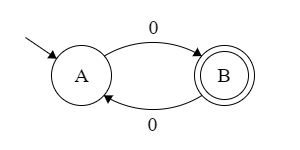
\includegraphics[width=150px]{03/odd_zeroes.png}

Proof that this automaton accepts the language:

\begin{itemize}
    \item This is the same automaton as in the previous exercise, but now the accept state is $B$, to accept an odd number of $0$'s.
\end{itemize}

\subsubsection{A perfect square number of \titlemath{$0$}'s}

\textbf{Gut feeling} (This is not yet proof!)

Not regular.

The issue here is going to be, that the length of the accepted words get further and further away from each other as the length of the words increases. We always need to keep track of how far away we are from the next accepted word, how many more $0$'s we need to finally accept. We would need separate states for each of these "$x$ number of $0$'s before we can accept", however $x$ could be arbitrarily large and we only have a finite number of states.

\textbf{Proof}

 Quite similar to \ref{3f1}, the $n+1$ words to use here are of the length of the first $n+1$ square numbers: $0 = 0^{1^2}$, $0000 = 0^{2^2}$, $0^9 = 0^{3^2}$, $0^{16} = 0^{4^2}$, $0^{5^2}$, $0^{6^2}$, $\dots$, $0^{(n+1)^2}$.
 
Then, the finishing of \ref{3f1} is a bit different:

When we find that for an $i\neq{}j$, both $0^{i^2}$ and $0^{j^2}$ end up in the same state $S$, the reasoning is a bit different. Without loss of generality, we can assume that $i<j$. If we were to continue $0^{i^2}$ from state $S$ with $2i+1$ more $0$'s, then the whole input would be $0^{i^2+2i+1} = 0^{(i+1)^2}$, which means that we should accept this word, so from state $S$, for $2i+1$ number of $0$'s we must reach an accept state.

However, this also means that when we continue $0^{j^2}$ (which remember, also arrives in $S$) with $2i+1$ $0$'s, so the word is $0^{j^2+2i+1}$, we will also arrive at the same accept state.

However $j^2+2i+1$ is not a square number. It is between two consecutive square numbers $j^2$ and $(j+1)^2 = j^2+2j+1$, but not equal to either of them:
\begin{itemize}
    \item $j^2 < j^2 + 2i + 1$, since $0<i$.
    \item $j^2 + 2i + 1 < j^2 + 2j + 1$, since $i<j$.
\end{itemize}

Thus, we found a word accepted by $M$, however not in $L$, which is a contradiction.

\subsubsection{A power of 2}

\textbf{Gut feeling} (This is not yet proof!)

Not regular, the situation is even worse than for square numbers, since powers of $2$ are even further spaced apart as the exponent continues to grow.

\textbf{Proof}

The $n+1$ words to be used are $0^{2^1}$, $0^{2^2}$, $0^{2^3}$, $\dots$, $0^{2^{n+1}}$.

Then similarly to the previous proof, when for $i\neq{}j$, $0^{2^i}$ and $0^{2^j}$ end up in the same state $S$, if we continue by $2^i$ more $0$'s, we should accept, since $0^{2\cdot{}2^i}$ is also a power of two number of $0$'s, however this means  $0^{(2^i + 2^i)}$ will also be accepted, but $2^i + 2^j$ is not a power of $2$, since $i\neq{}j$.